\pagelayout{wide} % No margins
\addpart{Introduction}
\labpart{introduction}
\pagelayout{margin} % Restore margins
\setchapterpreamble[u]{\margintoc}


\chapter{Introduction}
\labch{introduction}

\marginemptybox{3cm}
In today's world, software rules safety-critical systems such as nuclear power plants \sidecite{Krasner2021},
car engines \sidecite{Finch2009},
airplane control systems
\sidecite{Briere1993},
and medical devices \sidecite{Leveson1993}.
The reliability of these systems is based on their correctness.
Any failure or vulnerability in safety-critical software poses significant risks, potentially causing financial losses or threatening human safety.
Recent advances in software development have led to increasingly complex software systems.
As software grows in complexity, the likelihood of bugs also increases.
The effort and cost of fixing these bugs escalate with late detection, as illustrated in \reftab{effort-to-fix} \sidecite{White2017}, which shows the relative costs of fixing bugs at different development stages.
For safety-critical systems, detecting and addressing bugs before deployment is mandatory to ensure safety.

\begin{margintable}
  \caption{Cost of fixing bugs at different development stages \cite{White2017}.}
  \labtab{effort-to-fix}
  \centering
  \resizebox{\textwidth}{!}{
  \begin{tabular}{c c}
    \toprule
    \textsc{Bug Found at Stage} & \textsc{Cost to Fix} \\
    \midrule
    Requirements & 1x (definition) \\
    Architecture & 3x \\
    Design & 5-10x \\
    System Test & 10x \\
    Production & 10-100x \\
    \bottomrule
  \end{tabular}
  }
\end{margintable}

Beyond traditional software, machine learning-based software is increasingly being integrated into safety-critical systems, presenting new challenges to traditional assurance processes \sidecite{Googloe2023}.
Despite these challenges, the high standards for correctness in such systems remain the same, regardless of whether the software is traditional or machine learning-based.
Additionally, machine learning is also influencing societal decision-making in areas such as social welfare \sidecite{Larson2016}, criminal justice \sidecite{Buolamwini2018}, and healthcare \sidecite{Obermeyer2019}.
However, recent cases have demonstrated that machine learning software can inadvertently reproduce or even amplify biases present in the training data \cite{Buolamwini2018,Kay2015,Larson2016,Obermeyer2019}\phantomcite{Kay2015}.
In response of these risks, the European Commission proposed the Artificial Intelligence Act~\sidecite{Commission2021}, which aims to establish the first legal framework for machine learning software, with strict requirements to minimize the potential for discriminatory outcomes.
Therefore, detecting bugs and biases in machine learning software is crucial to ensure that it behaves as intended and does not cause harm to users.

% Beyond traditional software, also machine learning-based software is increasingly being used in safety-critical systems \sidecite{Googloe2023}.
% In such contexts, machine learning poses new challenges to traditional assurance processes.
% Nevertheless, the high standards for correctness in safety-critical systems remain the same, no matter of the software's nature.
% Furthermore, machine learning is increasingly impacting society by assisting or even automating decision-making in fields such as social welfare \sidecite{Larson2016}, criminal justice \sidecite{Buolamwini2018}, and healthcare \sidecite{Obermeyer2019}.
% However, recent cases have shown that such software can reproduce or even reinforce biases present in the training data \cite{Buolamwini2018,Kay2015,Larson2016,Obermeyer2019}\phantomcite{Kay2015}.
% In response to the rise of machine learning software based software, and thus the potential risks associated with it, the European Commission proposed the Artificial Intelligence Act~\sidecite{Commission2021}: a first legal framework on machine learning software, imposing strict requirements to minimize the risk of discriminatory outcomes.
% Overall, detecting bugs and bias in machine learning software is crucial to ensure that the software behaves as intended and does not harm users.


% Even more recently, the last advancements in artificial intelligence have led to the rise of large language models (LLMs) capable of generating software from natural language specifications.
% Agents like OpenAI's ChatGPT\sidenote{\rurl{chatgpt.com}} and Google's Gemini\sidenote{\rurl{gemini.google.com}} are gaining widespread use.
% Specifically designed for coding, GitHub Copilot\sidenote{\rurl{github.com/features/copilot}}. assists programmers within IDEs and has over a million subscribers\sidenote{\rurl{github.blog/news-insights/research/the-economic-impact-of-the-ai-powered-developer-lifecycle-and-lessons-from-github-copilot}}
% Despite their benefits, AI-generated code can introduce bugs as human-written code \sidecite{Asare2023}, making it crucial to use techniques that detect software errors or certify intended behaviors.

Overall, from more traditional to the latest machine learning-based software, detecting errors in safety-critical or high-stakes contexts is mandatory to ensure a correct software behavior.

\section{Software Quality}

Software quality measures how well software meets its requirements.
The most common method to ensure software quality is \emph{testing}.
The correct behavior of software is tested empirically for a finite number of inputs against a set of assertions specifying the functional requirements of the code.
However, testing has inherent limitations. For instance,
% It can only verify a program against functional requirements, which may be poorly defined and ambiguous, leading to inadequate testing.
exhaustive testing is impractical, and constraints on time and budget can further impact the process.
Mostly, testing cannot guarantee the absence of bugs\sidenote{``Program testing can be quite effective for showing the presence of bugs, but is hopelessly inadequate for showing their absence.'' -- \textcite{Dijkstra1976}}. \phantomcite{Dijkstra1976}
While in some cases deploying software with bugs and relying on patches to fix it is acceptable, \cf{} \reftab{effort-to-fix}, ensuring that software is free of bugs before deployment is necessary to avoid catastrophic consequences in safety-critical systems.

In contrast to testing, \emph{formal methods} provide rigorous mathematical guarantees about software correctness.
The idea of formally verifying software dates back to the late 1960s with program proofs and invariants from \sidetextcite{Floyd1967} and \sidetextcite{Hoare1969}.
Even earlier, formal methods can be traced to the work of \sidetextcite{Church1936} and \sidetextcite{Turing1937} on the foundations of computation.
According to software engineering practices, formal methods should be introduced early in the development lifecycle, enabling the verification of software properties at the design stage.

\begin{center}\em
  Why should formal methods complement other well-known, widely accepted, and user-friendly techniques such as testing?
\end{center}

To answer this question, consider the following examples where testing failed:

\begin{itemize}
\item The Ariane 5 rocket failure in 1996, caused by an integer overflow bug, resulted in a loss of \$370 million\sidenote{\rurl{esamultimedia.esa.int/docs/esa-x-1819eng.pdf}}.
\item The Therac-25 radiation therapy machine malfunctioned due to software bugs, resulting in patient deaths and serious injuries \sidecite{Leveson1993}.
\item The Toyota unintended acceleration case, where a stack overflow resulted in the death of 89 people and a lawsuit of \$1.2 billion\sidenote{\rurl{www.embeddedrelated.com/showarticle/1574.php}}.
\item A round-off error in the Patriot missile system caused the death of 28 people during the Gulf War\sidenote{\rurl{www.ima.umn.edu/~arnold/disasters/patriot.html}}.
\end{itemize}

These cases could have been avoided with formal methods.

Unlike testing, formal methods enable exhaustive search and detection of bugs that testing may miss.
System requirements are translated into formal specifications, which are mathematically verified to ensure the system's behavior aligns with real-world scenarios.
However, Rice's undecidability theorem \sidecite{Rice1953} states that all non-trivial program properties\sidenote{A property is trivial if it is true for all programs or false for all programs.} are undecidable, meaning there is no always terminating algorithm that can decide whether any program satisfies a non-trivial program property.
Consequently, formal methods either sacrifice: \emph{automation}, \emph{soundness}/\emph{termination}, or \emph{completeness}.
Based on this, formal methods are classified into three categories \sidecite{Cousot2010} (\cf{} \reffig{formal-methods-trade-offs}): \emph{theorem proving}, \emph{model checking}/\emph{symbolic execution}, and \emph{static analysis}.

\begin{marginfigure}
  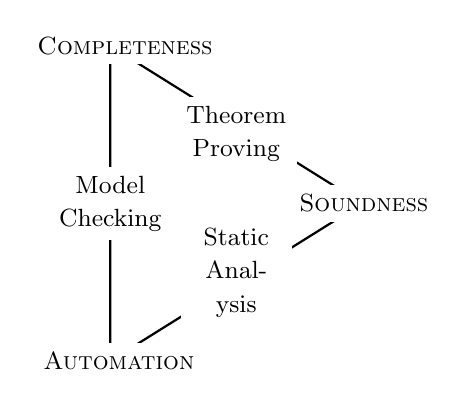
\begin{tikzpicture}[scale=0.8]
    % Draw the triangle
    \draw[thick] (0,0) -- (4,2.5) -- (0,5) -- cycle;

    % Place the vertices with blue squared borders
    \node[draw, fill=white, text width=1.7cm, align=center, draw=white] at (0,0) {\small \textsc{Automation}};
    \node[draw, fill=white, text width=1.6cm, align=center, draw=white] at (4,2.5) {\small \textsc{Soundness}};
    \node[draw, fill=white, text width=1.85cm, align=center, draw=white] at (0,5) {\small \textsc{Completeness}};

    % Place the edges' labels inside the edges
    \node[fill=white, text width=1.18cm, align=center] at (2,1.4) {\small Static Analysis};
    \node[fill=white, text width=1.5cm, align=center] at (0,2.5) {\small Model Checking};
    \node[fill=white, text width=1.3cm, align=center] at (2,3.6) {\small Theorem Proving};
\end{tikzpicture}
  \caption{Trade-offs in formal methods.}
  \labfig{formal-methods-trade-offs}
\end{marginfigure}

\paragraph{Theorem Proving.}
\index{Theorem Proving}

Theorem provers \sidecite{Nawaz2019} produce proofs of correctness using interactive tools, also called proof assistants, such as \textsc{Coq} \sidecite{Bertot2004}, \textsc{HOL Light} \sidecite{Harrison2009}, \textsc{Lean} \sidecite{Moura2021}, \textsc{Isabelle} \sidecite{Wenzel2008}, and \textsc{Agda} \sidecite{Bove2009}.
Theorem provers are complete and sound but not fully automated.
Indeed, user interaction is ultimately required to guide the proof search.
There are some attempts to automate theorem proving \sidecite{Sutcliffe2001} based on proof search strategies where the prover automatically search for the proof.
Nevertheless, the user interaction is still required whenever the proof search fails.
In this category of complete and sound methods also fall proof-oriented programming languages, such as \textsc{Dafny} \sidecite{Leino2010},  \textsc{F*} \sidecite{Swamy2016}, and \textsc{Why3} \sidecite{Filli_atre2013}.

\paragraph{Model Checking.}
\index{Model Checking}

Formal methods based on model checking \sidecite{Clarke1981,Queille1982} automatically explore the state space of a program's model to verify whether undesirable states are reachable.
Modern software model checkers trade termination for automation and completeness, as state-of-the-art software model checkers may not terminate.
When the answer is \emph{unknown}, indicating that the verification process halted on a timeout, the property may still be satisfied or violated, but the model checker was not able to determine it as the search space was too large.
However, model checking is complete because when the model checker answers that the property has been violated, a counterexample is provided.
\sidetextcite{Clarke2004} applied model checking to prove the correctness of ANSI-C programs.

\paragraph{Symbolic Execution.}
\index{Symbolic Execution}

Symbolic execution \sidecite{Baldoni2018} approaches perform abstract execution of programs to collect constraints on the program execution. During the abstract computation, variables with unknown values are represented symbolically and propagated through the program.
The collected constraints are then solved to verify whether an assertion is violated or not. As model checking, symbolic execution trades soundness for automation and completeness.
Tools like \textsc{KLEE} \sidecite{Cadar2008}, \textsc{BinSec} \sidecite{David2016}, and \textsc{PathFinder} \sidecite{Pasareanu2010} are based on symbolic execution.

\paragraph{Static Analysis.}

Static analysis verifies the program source code at some level of abstraction without user interaction.
This abstraction is sound but incomplete, meaning the analysis may report \emph{false alarms}, \ie, warnings that a correct program may be incorrect.
However, whenever the static analysis certifies the absence of a bug, the program is indeed bug-free.
In formal methods, the most common static analysis techniques are based on \emph{abstract interpretation}.

\paragraph{Abstract Interpretation.}
\index{Abstract Interpretation}

Abstract Interpretation \sidecite{Cousot1977} is a general theory for approximating program semantics, developed by Patrick and Radhia Cousot in the late 1970s (see \sidecite{Cousot2024a} for an historical view and \sidecite{Cousot2021} for a comprehensive overview).
Their framework is based on the observation that not all computational details are necessary to reason about program properties.
Instead, the program's semantics can be approximated by a simpler, more abstract model that facilitates automatic reasoning.

Over the past decade, abstract interpretation-based static analyses became part of the software development lifecycle of safety-critical systems.
For instance, the \textsc{Astrée} static analyzer \sidecite{Blanchet2003} is routinely used to ensure the absence of runtime errors in embedded synchronous C programs by Airbus.

We provide a formal introduction to abstract interpretation in \refch{abstract-interpretation}.
At the end of that chapter, we will illustrate the main results on a small idealized programming language.

\section{Input Data Usage}
\index{Input Data Usage}

Programming errors in software systems do not always result in crashes or runtime errors.
Sometimes, faulty programs produce plausible yet erroneous outcomes or unsafe behaviors.
Such bugs are hard to spot since they provide no clear indication that something went wrong.
A potential and common source of such errors is the misuse of input data, \ie, when an input variable has an unexpected impact on the program computation compared to the developers' expectations.

A notable example is the Reinhart and Rogoff article “Growth in a Time of Debt” \sidecite{Reinhart2010}, which claimed that economic growth is negatively correlated with public debt.
This article was heavily cited to justify austerity measures worldwide in the following years.
However, in 2013, \sidetextcite{Herndon2014} discovered that the authors had made a mistake in their Excel spreadsheet, leading to the erroneous conclusion.
One of the errors was the incorrect usage of the input value relative to Norway's economic growth in 1964, with an excessive weight in the average growth rate computation.

In data science and machine learning applications, where software involves long pipelines that filter, merge, and manipulate data, programming errors causing input variables to have more or less influence than expected are even more likely to occur.
Hence, it is essential to employ techniques that enhance confidence in the usage of input variables for data-driven applications.


In \arefpart{background}, \refch{input-data-usage} formally introduces input data usage, a program property that captures the \emph{qualitative} usage of input data in a program, as proposed by \textcite{Urban2018}.
We provide a hierarchy of semantics that precisely captures the input data usage property, abstracting unnecessary details.
Finally, we report an abstract semantics that captures syntactic dependencies between variables from \sidetextcite[][Section 10]{Urban2018}, used to approximate the input data usage property soundly.


\paragraph{Contributions}

In \refch{input-data-usage}, we extend the original definition of the input data usage to capture abstractions of output values, similarly to abstract non-interference \sidecite{Giacobazzi2018}, discussing relations between the two properties.
Such extension blends abstract non-interference with input data usage, providing a definition that works for non-deterministic programs natively without the need of a specialized program semantics.


\section{Quantitative Properties}
\index{Quantitative Information Flow}
Typically, program properties are qualitative: a program either satisfies a property or not.
This is not always sufficient for capturing the complexity of real-world requirements \sidecite{Smith2007}.
For instance, in program security, one fundamental requirement is protecting sensitive information confidentiality.
Secure information flow analysis questions whether a program could leak information about its secrets.
Non-interference, certifying that a program reveals no information about its secrets, is a classic secure information flow approach.
However, non-interference is too strict for many practical applications.
For example, in a digital election protocol, individual votes should be anonymous, but the final result needs to be revealed.
A password checker should not reveal the password but should indicate whether the password is correct.
These cases represent deliberate violations of non-interference necessary for the program to fulfill its purpose.

To address this limitation, quantitative properties are considered \sidecite{Smith2009}.
The key idea is to accept that a program may violate a property and compare such violation against a threshold.
Programs are classified as \emph{safe} or \emph{unsafe} based on the degree of violation, inducing a classification among programs based on how much safety they provide.

In the Reinhart and Rogoff case,
the error was not whether
the value of Norway's economic growth
was used
in the average computation
but rather how much it was used, \ie,
its impact was much higher than it should have been.
A quantitative analysis would have revealed that the impact of Norway's economic growth was too high, allowing the authors to correct the wrong conclusion.

\subsection{Quantitative Verification of Extensional Properties}[Extensional Properties]

\marginnote{\refch{quantitative-input-data-usage} and \refch{showcase} in \arefpart{extensional} are based on the work published at NASA Formal Methods
Symposium (NFM) 2024 \cite{Mazzucato2024b}.}
\marginnote{\formatmargincitation{Mazzucato2024b}}

In the first part of this thesis, we propose semantics-based static analysis techniques to quantify the impact of input variables on program computation.
In \refch{quantitative-input-data-usage}, we introduce a new formal framework based on abstract interpretation for reasoning about quantitative input data usage properties.
This framework can identify variables with disproportionate impact, certifying intended behavior or revealing potential flaws by matching developers' expectations with actual results.
We characterize the impact of an input variable with a notion of dependency between variables and program outcomes.
Our framework is parametric in the impact definition of choice.
%
We introduce a backward static analysis based on abstract interpretation, parametric in the impact definition, which infers a sound over-approximation of the impact of input variables.
% The analysis computes the input-output relations of a given program, then applies a computable implementation of the impact on the backward reachability analysis result.
This approach allows end-users to choose the impact that fits their needs, ensuring a targeted and customizable analysis.


\refch{showcase} demonstrates the quantitative framework's potential applications by evaluating our static analysis tool, \impatto\sidenote{\label{intro:impatto}\impattourl}, on six use cases.

\marginnote{\refch{quantitative-fairness} and \refch{evaluation-on-neural-networks} in \arefpart{extensional} are based on the work published at the 28th Static Analysis Symposium (SAS) 2021 \cite{Mazzucato2021}.}
\marginnote{\formatmargincitation{Mazzucato2021}}

In \refch{quantitative-fairness}, we extend the quantitative input data usage property to neural networks.
We propose two impact quantifiers for neural networks, addressing the challenges arising from the highly non-linear input space and measuring input features' fairness.
We refine the backward analysis to exploit parallel computations for better performance, employing a combination of forward and backward analysis.
The forward pass reduces the backward analysis's combinatorial explosion, partitioning the input space into subregions for easier parallelization.
\refch{evaluation-on-neural-networks} demonstrates the effectiveness of our approach on neural networks, showing that our method can identify input features with a disproportionate impact on the network's output, or quantify the fairness of neural networks.



\paragraph{Contributions}
The followings are the contributions of \arefpart{extensional}, consisting of \cref{ch:quantitative-input-data-usage,ch:showcase,ch:quantitative-fairness,ch:evaluation-on-neural-networks}:

\begin{itemize}
  \item In \refch{quantitative-input-data-usage}, we develop a theoretical framework by abstract interpretation to quantify the impact of input variables by considering three novel impact quantifiers.
  \item In \refch{quantitative-input-data-usage}, we present our static analysis and a possible abstract implementation of the impact instances.
  \item In \refch{showcase} our tool called \impatto{} showcases our approach against a set of six demonstrative programs.
  \item An artifact of \impatto{} comprehensive of \impatto's source code, documentation, and evaluation benchmarks is available on Zenodo\sidenote{\impattozenodo}.
  \item In \refch{quantitative-fairness}, we present two novel impact quantifiers for neural networks.
  \item In \refch{quantitative-fairness}, we propose an improved backward analysis that exploits parallel computations and achieves better precision by combining abstract domains.
  \item In \refch{evaluation-on-neural-networks}, we extended \impatto{} and \libra\sidenote{\libraurl} tools to evaluate our quantitative analysis on neural networks.
  \item An artifact extending \libra{} with the quantitative evaluation of fairness is available on Zenodo\sidenote{\librazenodo}.
\end{itemize}

\subsection{Quantitative Verification of Intensional Properties}[Intensional Properties]

\marginnote{\arefpart{intensional} is based on the work published at the 31st Static Analysis Symposium (SAS) 2024 \cite{Mazzucato2024c}.}
\marginnote{\formatmargincitation{Mazzucato2024c}}

\arefpart{intensional} focuses on the quantitative verification of intensional properties, \ie, properties that depend on the program's internal behavior, \eg, the number of iterations of a loop.
This part is divided into two chapters: the first one presenting the novel quantitative timing analysis, and the second one showing the experimental evaluation.

In \refch{quantitative-static-timing-analysis}, we consider the number of program iterations as the program outcome, capturing the impact of input variables on the global number of iterations.
Therefore, we are able to discover programming errors affecting iterations can degrade performance or introduce security vulnerabilities without functional errors.
For instance, unexpected input impacts on runtime could reveal sensitive information \sidecite{Wong2005}, posing security threats.
Even cryptographic programs are vulnerable to timing attacks, depending on implementation choices.
\sidetextcite{Kocher1996} demonstrated that public key cryptographic algorithms, like RSA, are susceptible to timing attacks, potentially leaking secret keys.

% Knowing the timing behavior of a program can certify intended behavior or reveal latent flaws by matching developers' expectations with actual program behavior.
For performance optimization, identifying input variables that significantly affect loop iterations helps developers focus on critical code segments \sidecite{Omar2017}.
Consequently, understanding the impact of input variables on runtime is paramount.
In this second part of the thesis, we focus on quantifying input variables' impact on loop iterations as an indicator of runtime behavior.

We leverage global loop bound analysis to derive an over-approximation of the global loop bound, encoding the quantification of input variables' impact as a linear programming problem.
Our approach blends syntactic and semantic information: generating invariants as linear constraints for accuracy and combining global loop bound analysis with syntactic dependency analysis \sidecite[][Section 10]{Urban2018} for scalability.

In \refch{sas24-eval}, we present \timesec\sidenote{\timesecurl}, a tool implementing our quantitative timing analysis.
We demonstrate its effectiveness in the Amazon Web Services \bignum{} cryptographic library\sidenote{\bignumurl}, certifying its immunity to timing side-channel attacks by showing no impact of input variables on loop iterations.
Additionally, we evaluate \timesec{} against programs from \svcomp\sidenote{\svcompurl}, a benchmark suite specifically designed for software verification tools.


\paragraph{Contributions}

The followings are the contributions of \arefpart{intensional}:

\begin{itemize}
  \item In \refch{quantitative-static-timing-analysis}, we propose a static analysis, employing a linear constraint abstract domain, global loop bound analysis, and linear programming encoding, to quantify the impact of input variables on loop iterations.
  \item In \refch{sas24-eval}, we present \timesec\sidenote{\timesecurl}, a tool implementing our quantitative timing analysis, and evaluate it against the \bignum{} cryptographic library\sidenote{\bignumurl} and programs from \svcomp\sidenote{\svcompurl}.
  \item An artifact of \timesec{} comprehensive of \timesec's source code and evaluation benchmarks is available on Zenodo\sidenote{\timeseczenodo}.
\end{itemize}

\frenchdiv

Related works are discussed at the end of each chapter, providing a comprehensive overview of the relevant literature.
At the end of the thesis, in \arefpart{conclusion}, we conclude the thesis with a summary and perspectives on future directions.

The next chapter shows the introduction in French language.
